%This file will be included in the ThesisMain Document as the experimentation
%section.

%Author: James Kelly
%Last Modified: 11-12-08

\begin{center}
\section{Theory}
\end{center}

The data from the stormwater discharge simulation trials support several elementary theories that successfully model and predict energy transfer outcomes. These concepts and models can in all liklihood be applied to any non-consolidated material  in a variety of flow scenarios. Two seperate approaches yield similar outcomes that are aligned with experimental results. Each approach offers the benefit of different conceptualizations. \\


\paragraph{Resistor-Capacitor Circuit Analogy}
The first of these scenarios involves modeling the vessel circuit as an electrical resistor-capacitor circuit. The conceptualization here stems from the analogy of thermal to electrical potential and is useful when considering specific consequences of heat loss. In this case, the applied voltage to the RC element is directly analogous to the difference between the reservoir temperature and the ambient temperature. This quantity is the total thermal potential and drives the transfer of energy between the fluid flow and the aggregate. 

\begin{figure}
\label{rctherm}
\begin{center}
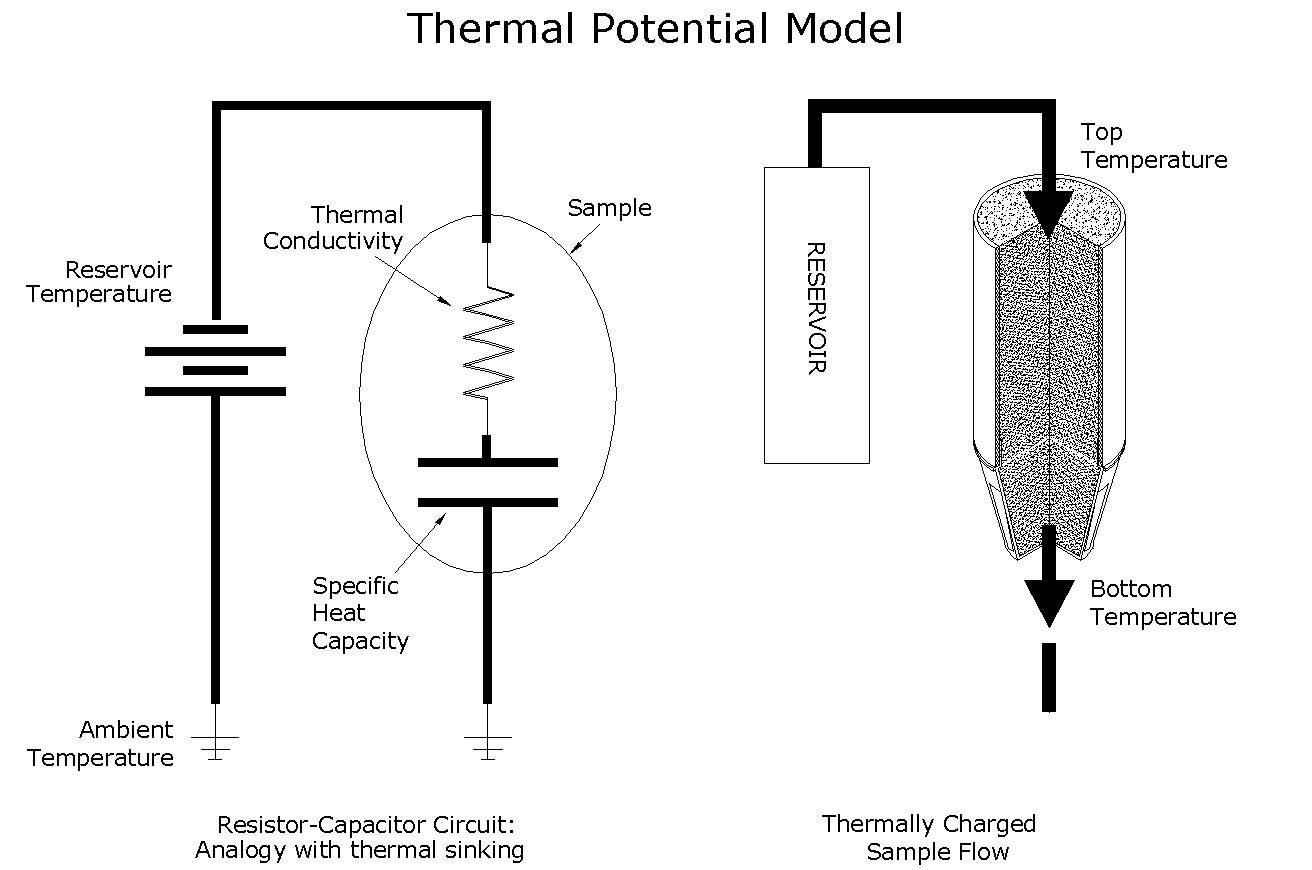
\includegraphics[scale=.25]{RCtherm.jpg}
\caption{An RC circuit is shown as a potential model for the sample vessel under thermal load.}
\end{center}
\end{figure}

Equation \ref{rc} models the voltage across the capacitor as an RC circuit charges \cite{elec}. In upholding the analogy, $V_{C}$ represents the temperature between the aggregate and the fluid flow at a time $t$. The second part of this theory section realizes that the temperature gradient between the top and bottom temperature sensors at a time $t$ is non-trivial and consequently the temperature between the rock and the fluid will vary not only with time but also with position. Therefore, in applying the RC circuit analogy, $V_{C}$ must be interpreted specifically as the average, bulk temperature difference between fluid and aggregate. 

\begin{equation}\label{rc}
 V_{C}(t)=V(1-e^{\frac{-t}{RC}})
\end{equation}

By equation (\ref{rt}), using $V$ as the total available thermal potential, $T_{o}=T[TOP]-T[AMBIENT]$, substituting the thermal resistivity $\kappa_{-1}$ for $R$, $c_{R}$ as the capacitance $C$ and letting $\sigma$ represent a dimensional constant with units of $\frac{kg}{m}$.
\begin{equation}\label{rcNew}
T(t)[R]=T_{o}(1-e^{x})\:\:\:\:\:\:\:x=\frac{\sigma t}{\left[\frac{c_{R}}{k}\right]}
\end{equation}

In the analysis of an RC circuit, the time constant $RC$ is used to characterize the response of the RC element. In the analog of that analysis, a new ``time constant'' appears in the exponent and is defined as the \emph{thermal moment}, $T_m$. This thermal moment characterizes how fast and how much heat can be transferred for an available potential, $T_{o}$. Let $\sigma=-\frac{R_{s}}{M_{s}}$ as the radius of the cobble and the total mass of the sample are necessary constants to compliment both $\kappa$ and $c_{R}$. 

\paragraph{Empirical Formulation from known parameters}

\begin{figure}
\label{slab}
\begin{center}
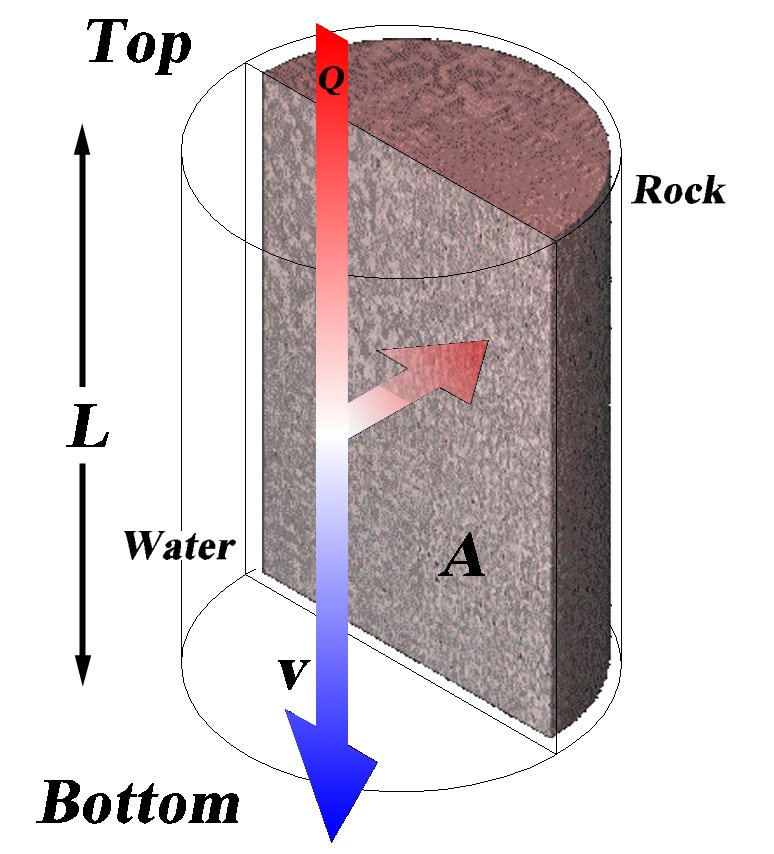
\includegraphics[scale=.25]{theorySlab.jpg}
\caption{A simplified model of the gravitationally charged experimental sample vessel where heat is exchanged between a hydraulic flow (water) and a thermal sinking sample (rock - aggregate)}
\end{center}
\end{figure}

The method that follows was developed by C.S. Thaxton as a means of developing a theoretical understanding of the heat exchange processes. The work here is presented as a theoretical base that was derived and ultimately supported by the data collected in this experimentation. 

The experiment can be theorized in a general scenario that is founded on Fourier's Law, and does not depend on the sample or test material being of a non-consolidated nature. In this scenario, the test material is modeled as a solid slab for simplicity in determining a thermal contact area $A$ and in considering a flow regime. Furthermore, all heat transferred is assumed to take place only through a conduction mechanism, and convective or radiative processes are not considered in this formalism \cite{theoryKern}.

At any differential vertical segment $dl$, Fourier's Law can is approximated as the following:
\begin{equation}\label{fouiers}
 \dot{Q}(L,t)=-\kappa A\;\frac{T(y,t)[W]-T(y,t)[R]}{R_{s}}
\end{equation}
Here, the aforementioned nomenclature holds, except instead of using a time-stepped temperature or energy value for numerical analysis, a differential is considered over both space and time, with $y$ representing a position along the sample's height. The gradient argument in Fourier's Law is assumed to be a finite distance between the water/rock interface and the center of the rock. It is therefore represented by the rock's characteristic radius $R_{s}$. Solving this equation by means of variable seperation and integration yields the following intermediate result.
\begin{equation}\label{Tbar}
\Delta Q_{net}=-\kappa\left(\dfrac{A}{R}\right) \int_{0}^{t_{f}} \left[ \dfrac{1}{L}\int_{0}^{L} T[WR](y,t)dy \right]dt\:=\:-\kappa\frac{A}{R}\int_{0}^{t_{f}}\bar{T}[WR](t)dt
\end{equation}
Where the bracketed term is the spatial average of $T(t)[WR]$ along $L$ and is numerically equivalent to equation (\ref{rt}):
\begin{equation}\label{spatialT}
 \bar{T}(t)[WR]=\frac{1}{L}\int_{0}^{L}T(y,t)[WR]dL\;=\;\dfrac{-\Delta T(t)[TB]}{\sum\Delta T(t)[TB]}\left(2T[TOP]-T[AMBIENT]\right)
\end{equation}

By considering the first law of thermodynamics and net heat transfer as was discussed in the experiment section, it's possible to theoretically arrive at the following differential equation\cite{theoryKern}:
\begin{equation}\label{tempdiffeq}
 \dot{T}(y,t)[WR]=-\frac{\kappa(c_{R}-c_{W})}{c_{R}c_{W}}\frac{A}{R}\;T(y,t)[WR]
\end{equation}
This is soluble with the following function:
\begin{center}
\begin{equation}\label{solution}
\begin{aligned}
 T(y,t)[WR]=&T(y,0)[WR]e^{-\sigma_{f} t}\\
 \sigma_{f}=&-\frac{A(c_{R}-c_{W})}{R_{s}c_{W}}\;T_m\\
 T_m=&\frac{\kappa}{c_{R}}\\
\end{aligned}
\end{equation}
\end{center}
Equation (\ref{tempdiffeq}) can be simplified by letting $y=L$ and considering just the bulk temperature change over the entire sample and by assuming that the intial temperature difference between water and rock is equivalent to the total available potential difference between reservoir and ambient temperatures \cite{theoryKern}, let $T(0)[WR]=T_{o}$:
\begin{equation}\label{tempdiffeq2}
 \dot{T}(t)[WR]=T_{o}e^{-\sigma_{f} t}
\end{equation}

This solution is aligned with the result from the Thermal Potential Model. Understanding how various parameters in each of the respective exponents needs to be studied. The exponential term in the Thermal Potential Model appears over simplified and the curve only matches well behaved heat flows. The aforementioned empirical theory expands to include another exponential term that accounts for interaction area of the flow and rock, in addition to flow rate. Because this supporting theory is still being developed, future research should seek to understand the relationships between various parameters, if there are parameters not accounted for or where the fundamental source of error lies in noted discrepancies. 

\begin{figure}
\label{rctherm}
\begin{center}
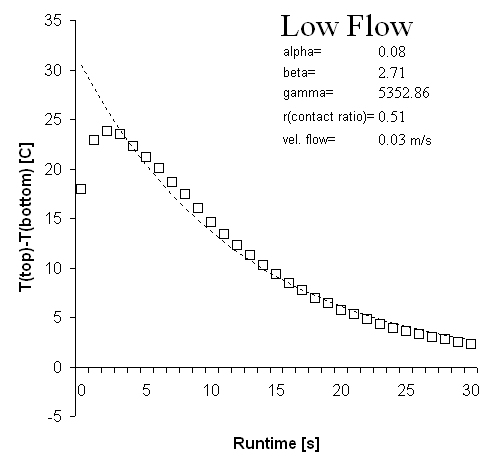
\includegraphics[scale=.25]{steellowFlow.jpg}
\caption{The empirically derived Fourier thermal model successfully predicts the temperature difference across the vessel on a control sample of mild steel balls. The time and length dependent temperature gradient that defines the vessel heat exchange is part of this model. The flow rate in this plot is rated low, or about 0.25 L/s.}
\end{center}
\end{figure}

%This is aligned with the result from the thermal potential modeling and RC circuit comparison. If we let both exponents, $\sigma_{RC}$ and $\sigma_{f}$ be equal, 
%\begin{equation*}
% \sigma_{RC}=\sigma_{f}
% T_{m}\;\frac{A(c_{R}-c{W})}{R_{s}(c_{W}}\;=\;T_{m}\;-\frac{R_{s}}{M_{s}}
%\end{equation*}



 



